
% CHAPTER:  1
% (Note: cannot have a footnote on a word within the \chapter{} construct, it does not work)
\newcommand{\s}{$_{\rm s}$}
\newcommand{\kms}{km~s$^{-1}$}
\newcommand{\msun}{{\it M}$_{\odot}$}
\newcommand{\lsun}{{\it L}$_{\odot}$}
\newcommand{\mear}{{\it M}$_{\oplus}$}
\newcommand{\etal}{{\it et al.}}
\newcommand{\ie}{{\it i.e.}}
\newcommand{\eg}{{\it e.g.}}
\newcommand{\be}{\begin{equation}}
\newcommand{\ee}{\end{equation}}
\newcommand{\magarc}{{\rm mag\,arcsec$^{-2}$}}
\newcommand{\MK}{{{\rm M}_{\rm ext,K}-5\log h}}
\newcommand{\ri}{{$r_{21}$}}
\newcommand{\ra}{$R_A$}
\newcommand{\vobs}{{v_{\rm obs}}}
\newcommand{\kmsMpc}{km~s$^{-1}$ Mpc$^{-1}$}
\newcommand{\h}{$h_{70}$}
\newcommand{\vpec}{v_{\rm pec}}
\newcommand{\like}{{\mathcal L}}
\newcommand{\vs}{\vspace*{5pt}}
\newcommand{\continued}{ (Continued)}

\newcommand{\ferengi}{\textsc{ferengi}}
\newcommand{\hst}{\textit{HST}}
\newcommand{\hubble}{\textit{Hubble Space Telescope}}
\newcommand{\subaru}{\textit{Subaru}}
\newcommand{\sextractor}{\textsc{SExtractor}}
\newcommand{\galapagos}{\textsc{Galapagos}}
\newcommand{\galfit}{\textsc{GALFIT}}
\newcommand{\gimtwod}{\textsc{GIM2D}}
\newcommand{\sersic}{S\'{e}rsic}






% Galaxy Zoo
\newcommand{\ffeatures}{$f_{\rm features}$}
\newcommand{\ffeaturesz}{$f_{\mathrm{features,}z}$}
\newcommand{\ffeaturesrest}{$f_{\mathrm{features,}z=0.3}$}
\newcommand{\ffeaturesdebiased}{$f_{\mathrm{features,debiased}}$}
\newcommand{\fbest}{$f_{\mathrm{features,best}}$}
\newcommand{\fodd}{$f_{\mathrm{odd}}$}
\newcommand{\fbar}{$f_{\mathrm{bar}}$}
\newcommand{\fclumpy}{$f_{\mathrm{clumpy}}$}
\newcommand{\fsmooth}{$f_{\rm smooth}$}
\newcommand{\fartifact}{$f_{\rm artifact}$}

\newcommand{\fHI}{f_{\rm HI}}
\newcommand{\zsim}{$z_{\mathrm{sim}}$}

% Bands

\newcommand{\Bband}{$B_{435W}$}
\newcommand{\Vband}{$V_{606W}$}
\newcommand{\iband}{$i_{775W}$}
\newcommand{\Iband}{$I_{814W}$}
\newcommand{\zband}{$z_{850LP}$}

% GZH subsamples

\newcommand{\main}{\texttt{main}}
\newcommand{\faded}{\texttt{faded}}
\newcommand{\recolored}{\texttt{recoloured}}
\newcommand{\goods}{\texttt{goods-shallow}}
\newcommand{\stripe}{\texttt{stripe-82-single}}
\newcommand{\coadd}{\texttt{stripe-82-coadd}}
\newcommand{\redshifted}{\texttt{redshifted}}
\newcommand{\simagn}{\texttt{simulated-agn}}



\chapter{Using FERENGI to correct \ffeatures{} for redshift-induced classification bias}
\label{chap:ferengi}

\subsection{Intro}
\label{ssec:ferengi_Intro}
%% motivate importance of f_features in selecting morphological samples for population studies, and introduce the bias induced in the measurement as a function of redshift 

The GZ vote fraction \ffeatures{} plays a crucial role in the majority of science cases that use Galaxy Zoo classifications. It represents the fraction of users who answered ``feature or disk'' to the first question in the decision tree, and is used to distinguish elliptical/spheroidal galaxies from those with features. Many studies aim to measure the popluation of galaxies exhibiting certain features such as bars (examples), spiral arms (examples), [dump stuff in this list]. In each of these, \ffeatures{} is necessary for creating the sample of galaxies which could potentially contain the feature in question. This is typically acheived by setting a cut, such that all galaxies with \ffeatures{} greater than that threshold are considered to be candidates for that study.

While \ffeatures{} is not a true probability, the measurement is intended to be consistent among all galaxies; that is, two galaxies with similar \ffeatures{} values should have similar likelihoods of being featured (or not featured). This has been shown to be true at low redshift by comparing the \ffeatures values to expert classifications (reference Willet et al. 2013); there is a strong correlation between this vote fraction and whether the galaxy was expertly classified as a disk or an elliptical [expand on what W13 actually did.].    

For distant galaxies, however, we observe that \ffeatures{} is not consistant with nearby galaxies. As galaxies are observed at higher redshift, the images are inherently less resolved, and smaller features are more difficult to identify. This causes in a decrease in \ffeatures{} than what would be expected if the galaxy had been observed at $z=0$. Figure [make a figure] shows this effect: [describe some figure, probably a bunch of galaxies that are obviously spirals but with very diff. ffeatures values at diff. redshifts.] Therefore, two identical galaxies, imaged at different redshift, may have small to drastic differences in their \ffeatures{} measurement. In order to keep \ffeatures{} a value correlated with the likelihood of having features that is consistent for \emph{all} galaxies, this bias must be corrected. 

A method for correcting redshift bias in the GZ vote fractions was developed and implemented in prior Galaxy Zoo projects (cite GZ1 and GZ2), which contained nearby ($z<0.2$) galaxies imaged by the SDSS. A correction factor to the classification fractions measured at the higher redshifts was applied by matching the mean vote fractions of those at the lowest redshift. This technique was valid under the assumption that, within this redhisft range, there would be no cosmological evolution of galaxies, and therefore any change in the mean vote fraction for any morphology with redshift was purely due to this observational bias, and not due to a genuine difference in morphological populations. 

In GZH, the redshift range is large enough that cosmological evolution of the morphologies of galaxies is expected, and therefore the previous method of correcting redshift-bias will not work. Instead, we have developed a new method of measuring the change in \ffeatures{} as a function of redshift using a set of simulated \ferengi{} images of galaxies, described in the next section. These images have been classified by volunteers in Galaxy Zoo in the same way as the GZH sample. This chapter will describe how we measure a correction factor for \ffeatures{} using these data as a function of redshift at fixed surface brightness, and apply the correction to the GZH sample. 


\subsection{The FERENGI sample}

\subsection{Measuring the drop in \ffeatures{} as a function of $z$ and $\mu$ using FERENGI data}
\subsubsection{Identifying ``correctable'' and ``lower limit'' samples.}

The objective is to use the simulated data from \ferengi{} to predict, for a galaxy imaged at a redshift $z$, and with a measured \ffeaturesz{} value, what its \ffeatures{} value \emph{would have been} if it had been viewed at $z=0.3$. This predicted value is defined as the ``debiased' vote fraction \ffeaturesdebiased, and is calculated by applying a correction to the measured value of \ffeatures.

The amount that a galaxy's \ffeatures{} vote fraction must be corrected is assumed to primarily depend on the apparent size and brightness of the galaxy. As described in \ref{ssec:ferengi_Intro}, these factors will affect the overall clarity of the image viewed by the GZ volunteers, which in turn affects the likelihood of being able to identify distinct feature. The apparent size and brightness are controlled by both instrinsic parameters (absolute size and luminosity), and extrinsic (distance to the galaxy). The change in \ffeatures{} then is measured as a function of redshift ($z$, an extrinsic freature, measuring distance to the galaxy), and surface brightness ($\mu$, an intrinsic feature, taking into account both brightness and size).   

Figure~\ref{fig:f_vs_f} shows the change in \ffeatures{} for \ferengi{} galaxies in bins of redshift and surface brightness. Points in each $z,\mu$ represent individual \ferengi{} galaxies. On the x-axis of each bin is the value of \ffeatures{} measured in that galaxy's $z=0.3$ image (the lowest redshift of the simulated images). On the y-axis of each bin is the value of \ffeatures{} measured in that galaxy's $z=z$ image, where $z$ corresponds to the redshift associated with that bin. As predicted, the value of \ffeatures{} measured at a higher redshift, $z$, is, in general, \emph{lower} than the value measured at lower redshift, $z=0.3$, \emph{for the same galaxy}. This effect is strongest as redshift increases (to the right in Figure~\ref{fig:f_vs_f}) and as surface brightness decreases (upwards in Figure ~\ref{fig:f_vs_f}). 

% Figure - big ass plot
\begin{figure}
\begin{center}
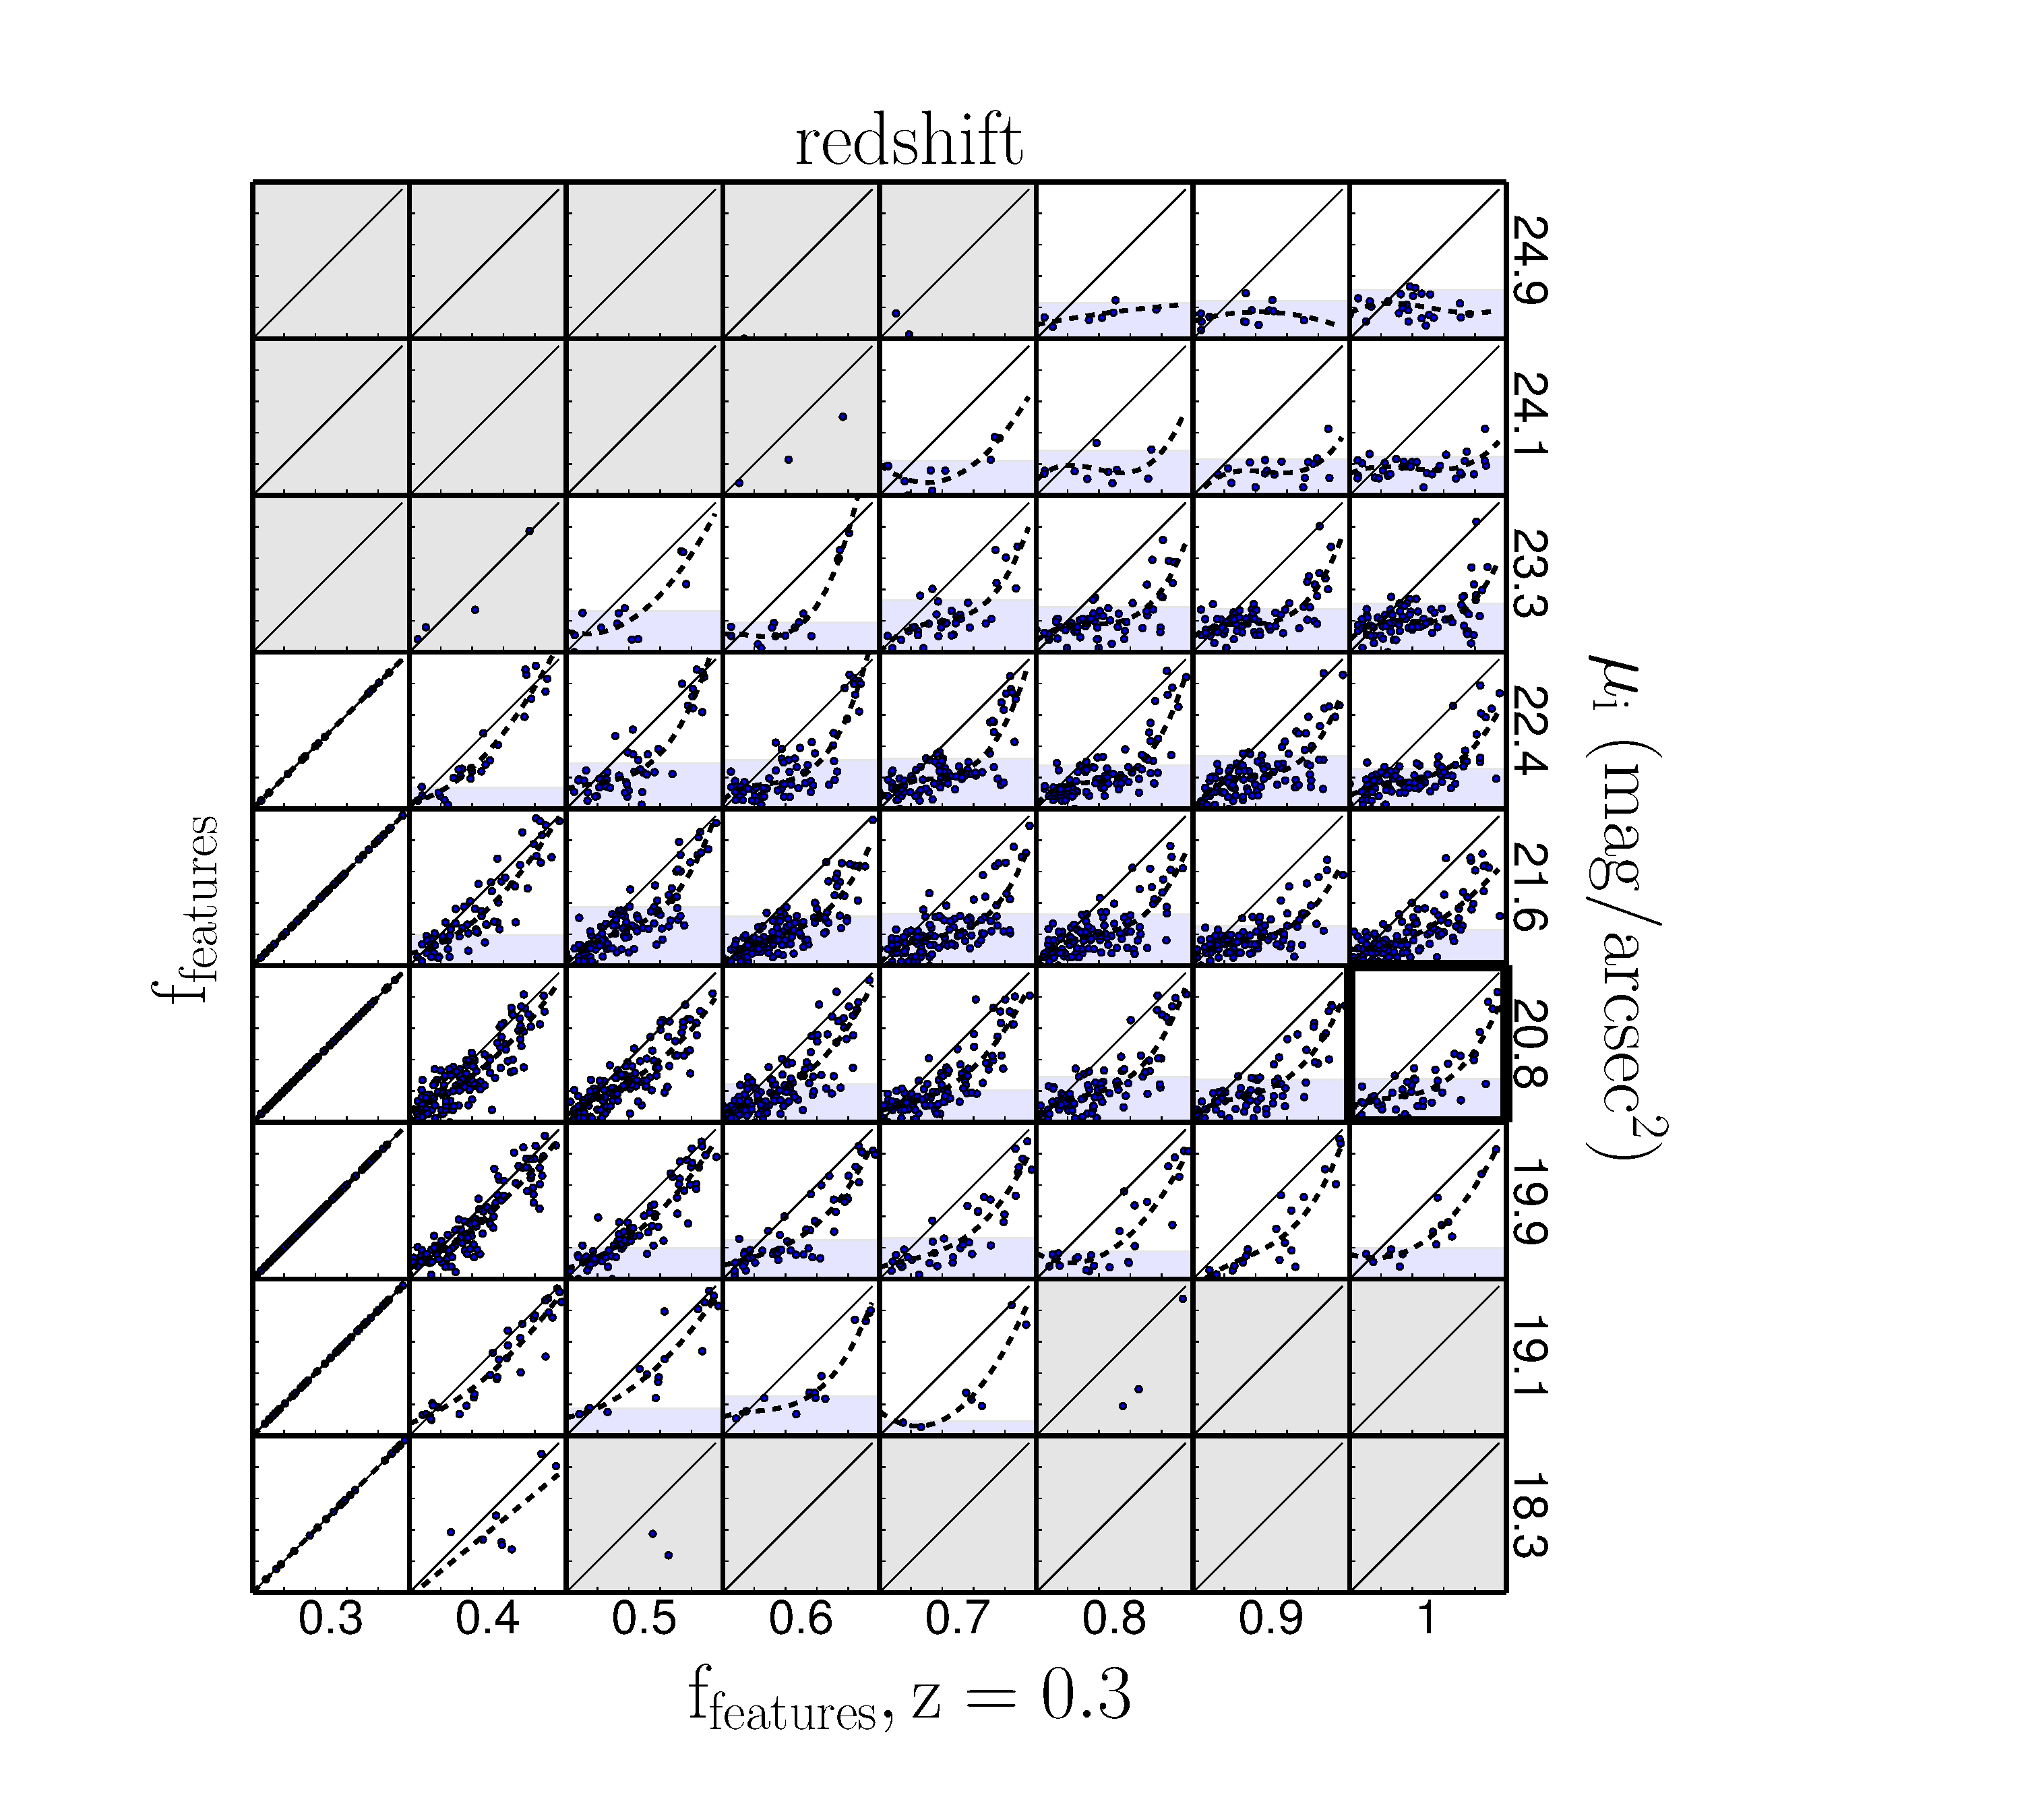
\includegraphics[scale=0.42]{figures/p_vs_p_SB_redshift.pdf}
\caption{Effects of redshift bias in 3,449~images in the \ferengi{} sample.
Each point \emph{in a given redshift and surface brightness bin} represents a
unique galaxy. On the $y$-axis in each bin is the \ffeatures{} value of the
image of that galaxy redshifted to the value corresponding to that redshift
bin. On the $x$-axis is the \ffeatures{} value of the image of the same galaxy
redshifted to $z=0.3$. The dashed black lines represent the best-fit
polynomials to the data in each square. The solid black line represents
\ffeaturesz=\ffeaturesrest. Regions in which there is a single-valued
relationship between \ffeatures{} at high redshift and at $z=0.3$ are white;
those in which there is not are blue, and those with not enough data ($N<5$)
are grey. A larger version of the bin outlined at $z=1.0$ and $20.3 < \mu <
21.0$ $\rm (mag/arcsec^2)$ is shown in Figure~\ref{fig:f_vs_f_zoom}.}
\label{fig:f_vs_f}
\end{center}
\end{figure}

% Figure - small ass plot
\begin{figure}
\centering
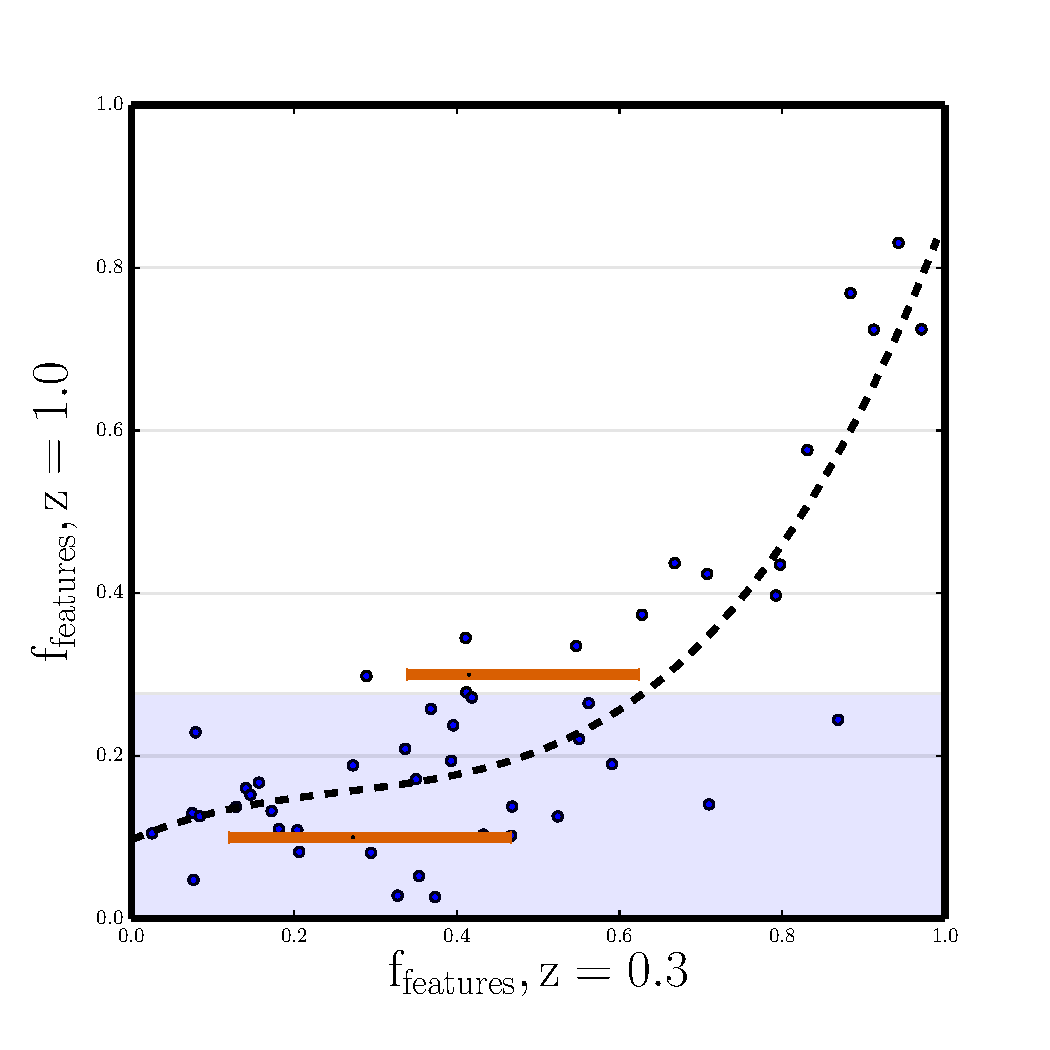
\includegraphics[width=0.7\textwidth]{figures/z1_mu20_subplot2.pdf}
\caption{A larger version of the dark-outlined square in Figure~\ref{fig:f_vs_f}, containing
\ferengi{} galaxies that have been artificially redshifted to $z=1.0$ and have
surface brightnesses between $20.3 < \mu < 21.0$ $\rm (mag/arcsec^2)$. The orange bars represent the inner
68\% (1$\sigma$) of the uncorrectable \ffeatures{} quantiles, which are used
to compute the limits on the range of debiased values.}
\label{fig:f_vs_f_zoom}
\end{figure}

A reliable predicted value can be obtained so long as
the relationship between \ffeaturesz{} and \ffeaturesrest{} is single-valued;
that is, for a given \ffeaturesz, there is exactly one corresponding value of
\ffeatures{} at $z=0.3$. Unfortunately, this is \emph{not} always the case. Figure~\ref{fig:f_vs_f_zoom} shows \ffeatures{} measured at $z=1$ vs \ffeatures{} measured at $z=0.3$ for \ferengi{} galaxies with average surface brightnesses $<\mu>=20.8$ (a zoomed-in version of the dark outlined bin in Figure~\ref{fig:f_vs_f}). This figure shows that if the value of \ffeatures{} measured for a galaxy at $z=1$ is particularly low, there is a wide range that \ffeatures{} could have been if measured at $z=0.3$. Therefore, a low measured value of \ffeatures{} at high redshift could represent two morphological types of galaxies: 1) The galaxy has no distinguishable features and may be classified as a smooth elliptical, or 2) the galaxy \emph{does} have features, but these have become blurred and too difficult to detect at high redshift. 

It is important to identify such regions of surface brightness/redshift/\ffeatures{} space since vote fractions cannot be confidentely corrected to a single value for galaxies in these regions. The criteria for determining whether a region of this space is single-valued, and therefore correctable, is as follows: In each surface brightness and redshift bin, the relationship between \ffeaturesz{} and \ffeaturesrest{} is modelled by fitting the data with polynomials of degress n=3,2, and 1, and using the best formal fit out of the three as measured by the sum of the residuals. These fits are shown as the dashed black lines in Figures~\ref{fig:f_vs_f} and~\ref{fig:f_vs_f_zoom}. Flat regions of the bins are areas in which there is \emph{not} a clear single-valued relationship between \ffeaturesz{} and \ffeaturesrest{}. This is quantified by measuring the slope of the best-fit polynomial to the vote fractions; regions of the bins with a slope less than 0.4 are considered \emph{not} one-to-one, and therefore \ffeaturesz{} cannot be boosted to its \ffeaturesrest{} value. These are colored blue in Figure~\ref{fig:f_vs_f} and are referred to as the \textit{lower limit} sample, because the most stringent correction available is that the weighted \ffeatures{} is a lower limit to the true value. 

The unshaded regions of Figure\ref{fig:f_vs_f_zoom} define descrete ranges of redshift, surface brightness, and \ffeatures{} within which a galaxy must lie in order for the debiased vote fraction to be confidentely applied. While the appropriate correctable regions were defined as discrete bins, the true correctable region is assumed to be a smooth function of $z, \mu,$ and \ffeatures{}. To define this smooth space, a convex hull was calculated to enclose the correctable and lower-limit \ferengi{} galaxies in the $z-\mu-$\ffeatures{} space (see Figure~\ref{fig:hull}). The space defined by this hull was used to ultimately separate the GZH galaxies into correctable samples (those for which a correction to \ffeatures{} can confidentely be applied, see next section) and lower-limit samples (those for which a single-valued correction cannot be applied). The final categorization of the GZH sample, split by imaging survey, is shown in Table~\ref{tab:hubble_debiasable}. 
% Figure - convex hull
\begin{figure}
\centering
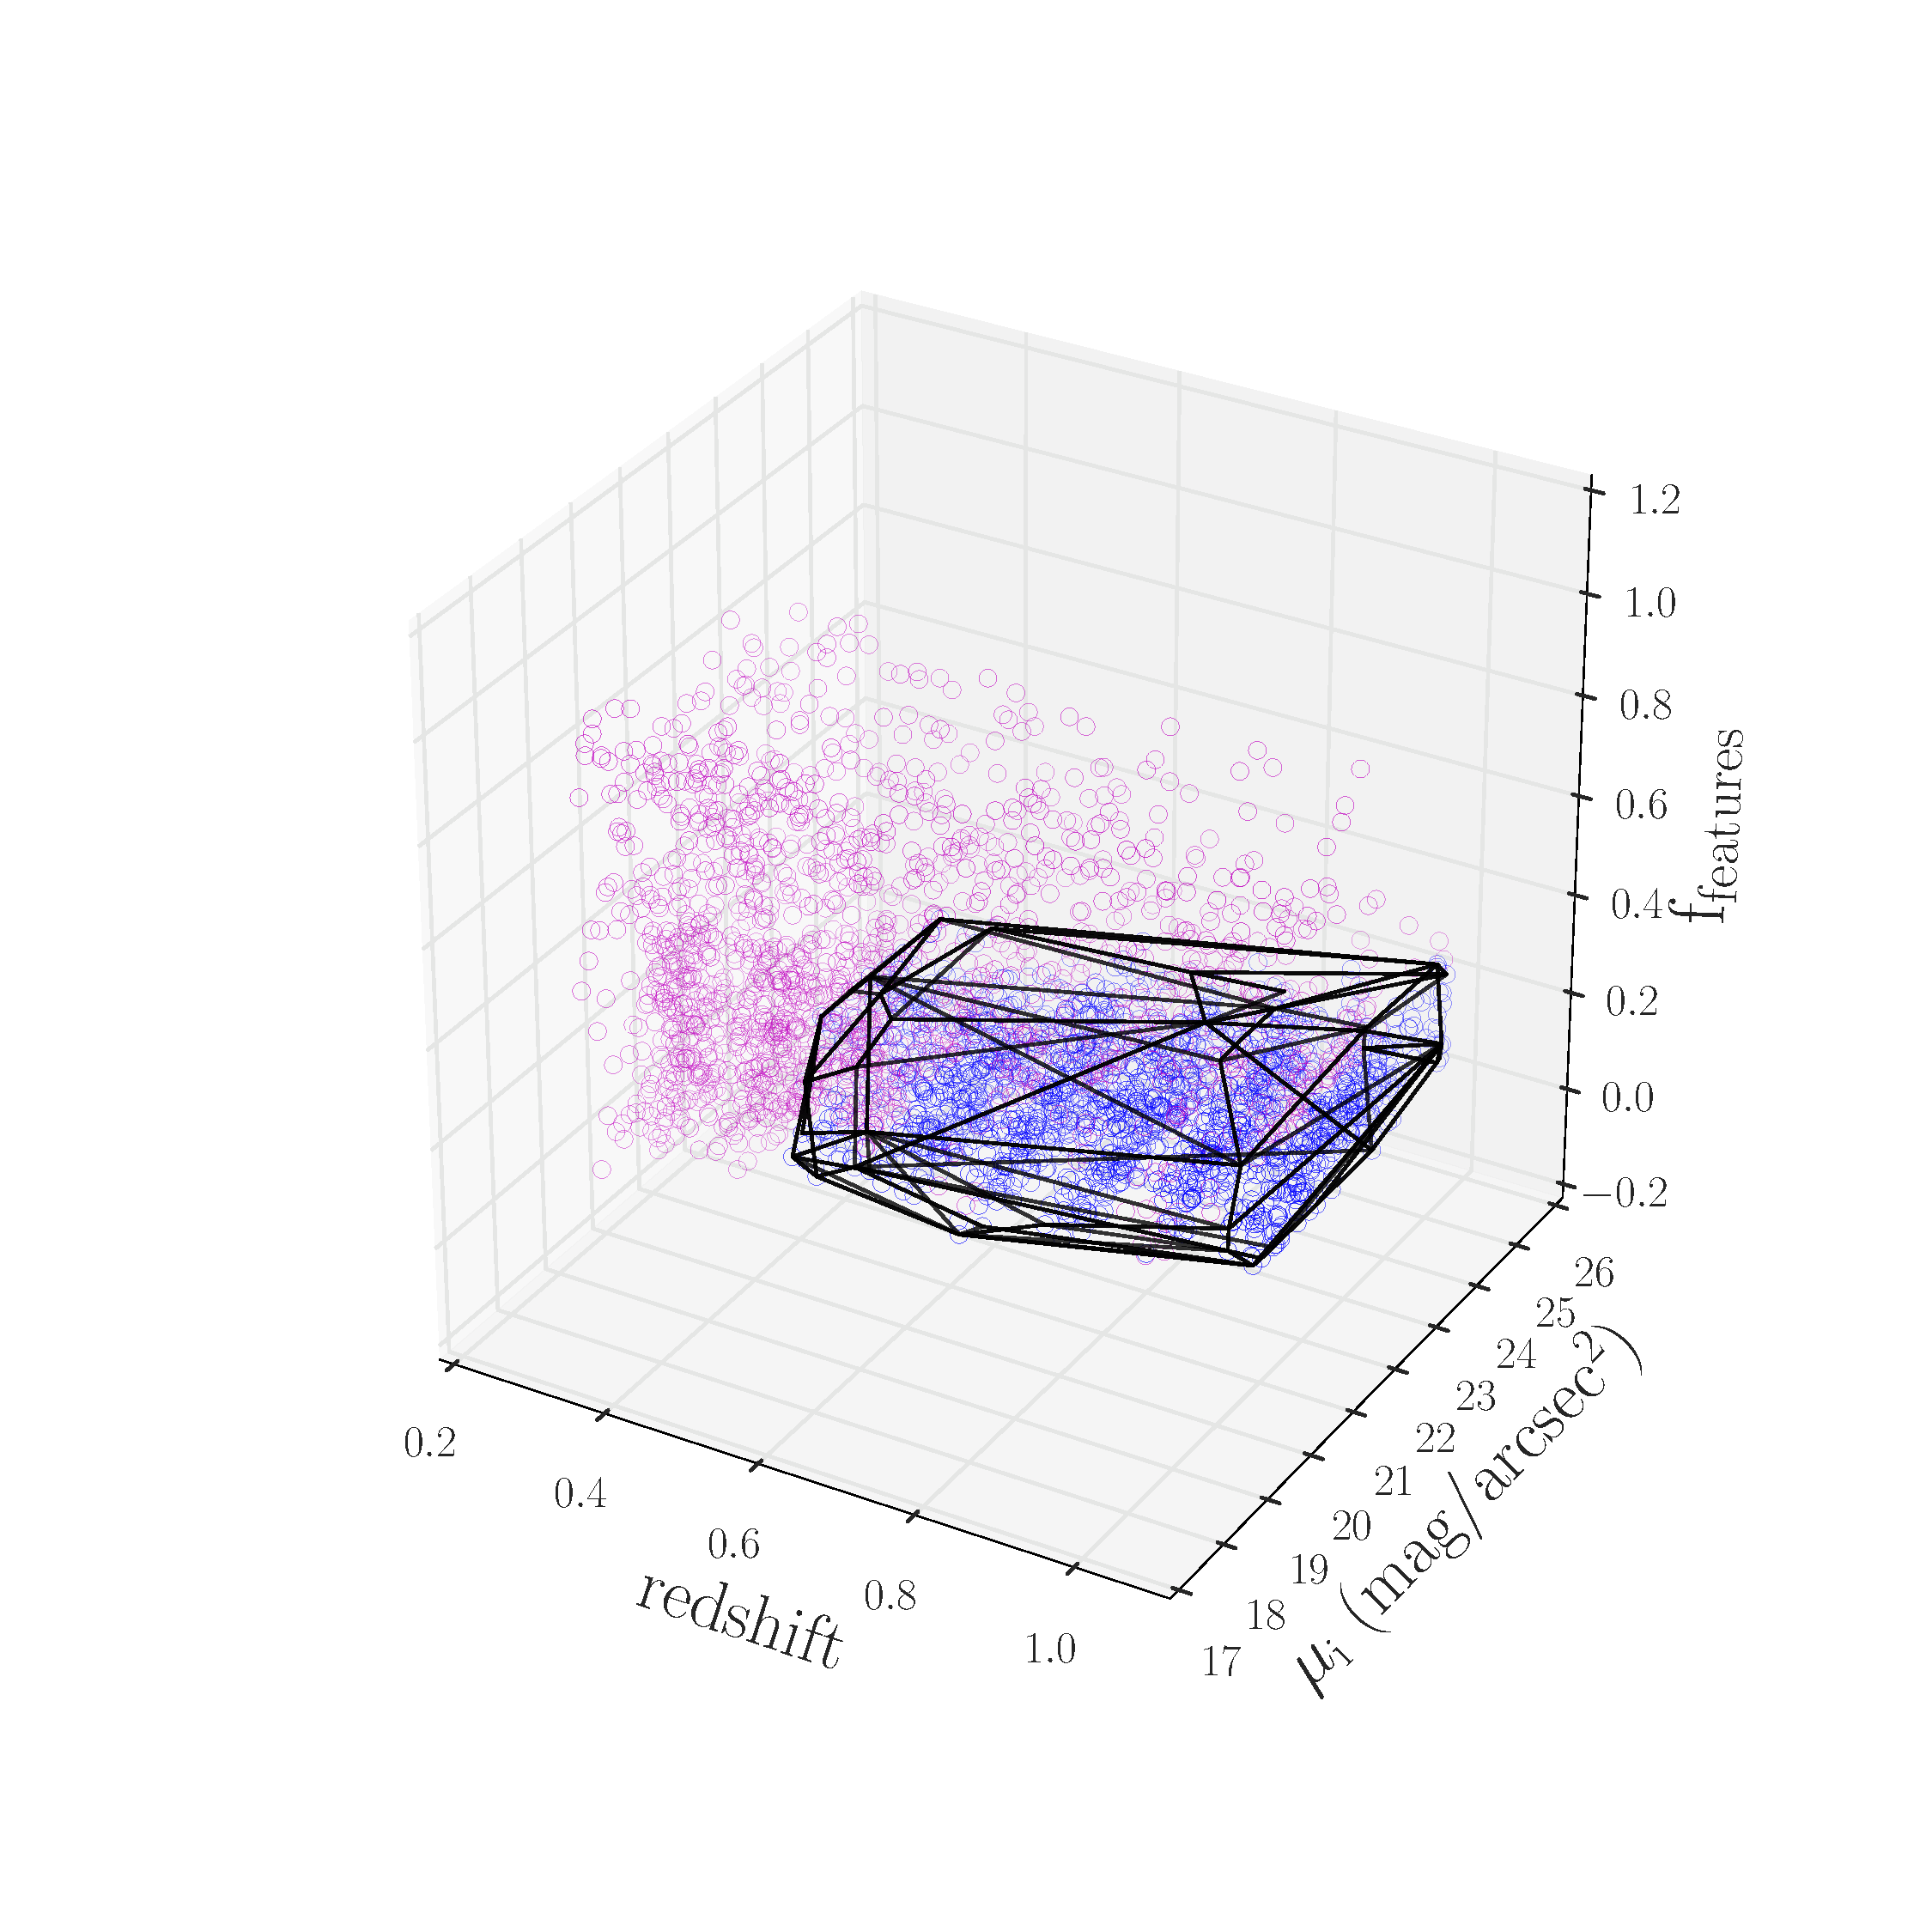
\includegraphics[width=\textwidth]{figures/convex_hull.pdf}
\caption{The final separation of the correctable and lower-limit samples in redshift/surface brightness/\ffeatures{} space.\textbf{Pink} points are all \ferengi{} galaxies in the \textbf{unshaded} regions of Figure~\ref{fig:f_vs_f}. \textbf{Blue} points are all \ferengi{} galaxies in the \textbf{blue shaded} regions of Figure~\ref{fig:f_vs_f}. The solid black line is the convex hull which encloses the uncorrectable points and defines the region of the lower-limit sample. }
\label{fig:hull}
\end{figure}



%Table: distribution of correction types for HST
\begin{table*}
\caption{Number of correctable galaxies for the top-level task in GZH, split by \hst{} survey.}\label{tab:hubble_debiasable}
\begin{tabular}{lcrrrrr|r}
\hline\hline
                                   & Correction type & AEGIS   & COSMOS & GEMS  & GOODS-N & GOODS-S  &  Total  \\
                                   &                 &         &        &       & 5-epoch & 5-epoch  &         \\
\hline
correctable                        & 0               & 2,908   & 21,169 & 2,802 & 1,459   & 1,189    &  29,527 \\
lower-limit                        & 1               &   833   &  5,169 & 1,021 & 1,377   & 1,267    &   9,667 \\
no correction needed ($z \le 0.3$) & 2               &   955   & 10,870 & 1,175 &   415   &   400    &  13,815 \\ 
not enough information (NEI)       & 3               & 2,677   & 43,058 & 3,559 & 2,077   & 2,184    &  53,555 \\
no redshift information            & 4               & 1,134   &  4,688 &   530 &   687   &   102    &   7,141 \\
\hline
total                              &                 & 8,507   & 84,954 & 9,087 & 6,015   & 5,142    & 113,705 \\
\hline\hline
\end{tabular}
\end{table*}




For the ``lower limit'' galaxies, since a single debiased \ffeatures{} value cannot be confidentely assigned, a \emph{range} of debiased values is estimated. In each $z,\mu$ bin in Figure~\ref{fig:f_vs_f}, the spread of intrinsic values of \ffeaturesrest{} for five quantiles of observed \ffeatures{} is computed - these are denoted by the gray lines in the close-up Figure~\ref{fig:f_vs_f_zoom}. The range of intrinsic values of \ffeatures{} is defined by the upper and lower 1 $\sigma$ limits, enclosing the inner 68\% of the data; this is represented by the orange bars in Figure~\ref{fig:f_vs_f_zoom}. For any galaxy which cannot be directly debiased, these ranges are used to denote the upper and lower limits on the expected values \ffeaturesrest{} as a function of the observed \ffeatures{}. 

\subsubsection{Computing debiased \ffeatures{} for the ``correctable'' sample using the $\zeta$ equation}

For the ``correctable'' sample of simulated \ferengi{} galaxies, an equation is derived to model the dropoff in \ffeatures{} with redshift for each galaxy. Such a model is assumed to have the following criteria: (1) For a given galaxy, \ffeatures{} should decrease relative to its \ffeaturesrest{} as redshift increases. (2) The corrected \ffeatures{} value must be contained within 0 and 1, since it is a fraction. (3) The degree of dropoff may depend on the surface brightness of the galaxy. Given these three assumptions, a simple exponential function was derived:

\begin{equation}
f_{\mu,z} = 1 - (1 - f_{\mu,z=0.3})e^{\frac{z-z_0}{\hat\zeta}}
\label{eqn:fzeta}
\end{equation}

where $f_{\mu,z=0.3}$ is the vote fraction at the lowest redshift in the artificially-redshifted \ferengi{} sample ($z_{0}=0.3$). $\zeta$ is a parameter that controls the rate at which \ffeatures decreases with redshift. 

\begin{figure*}
\center
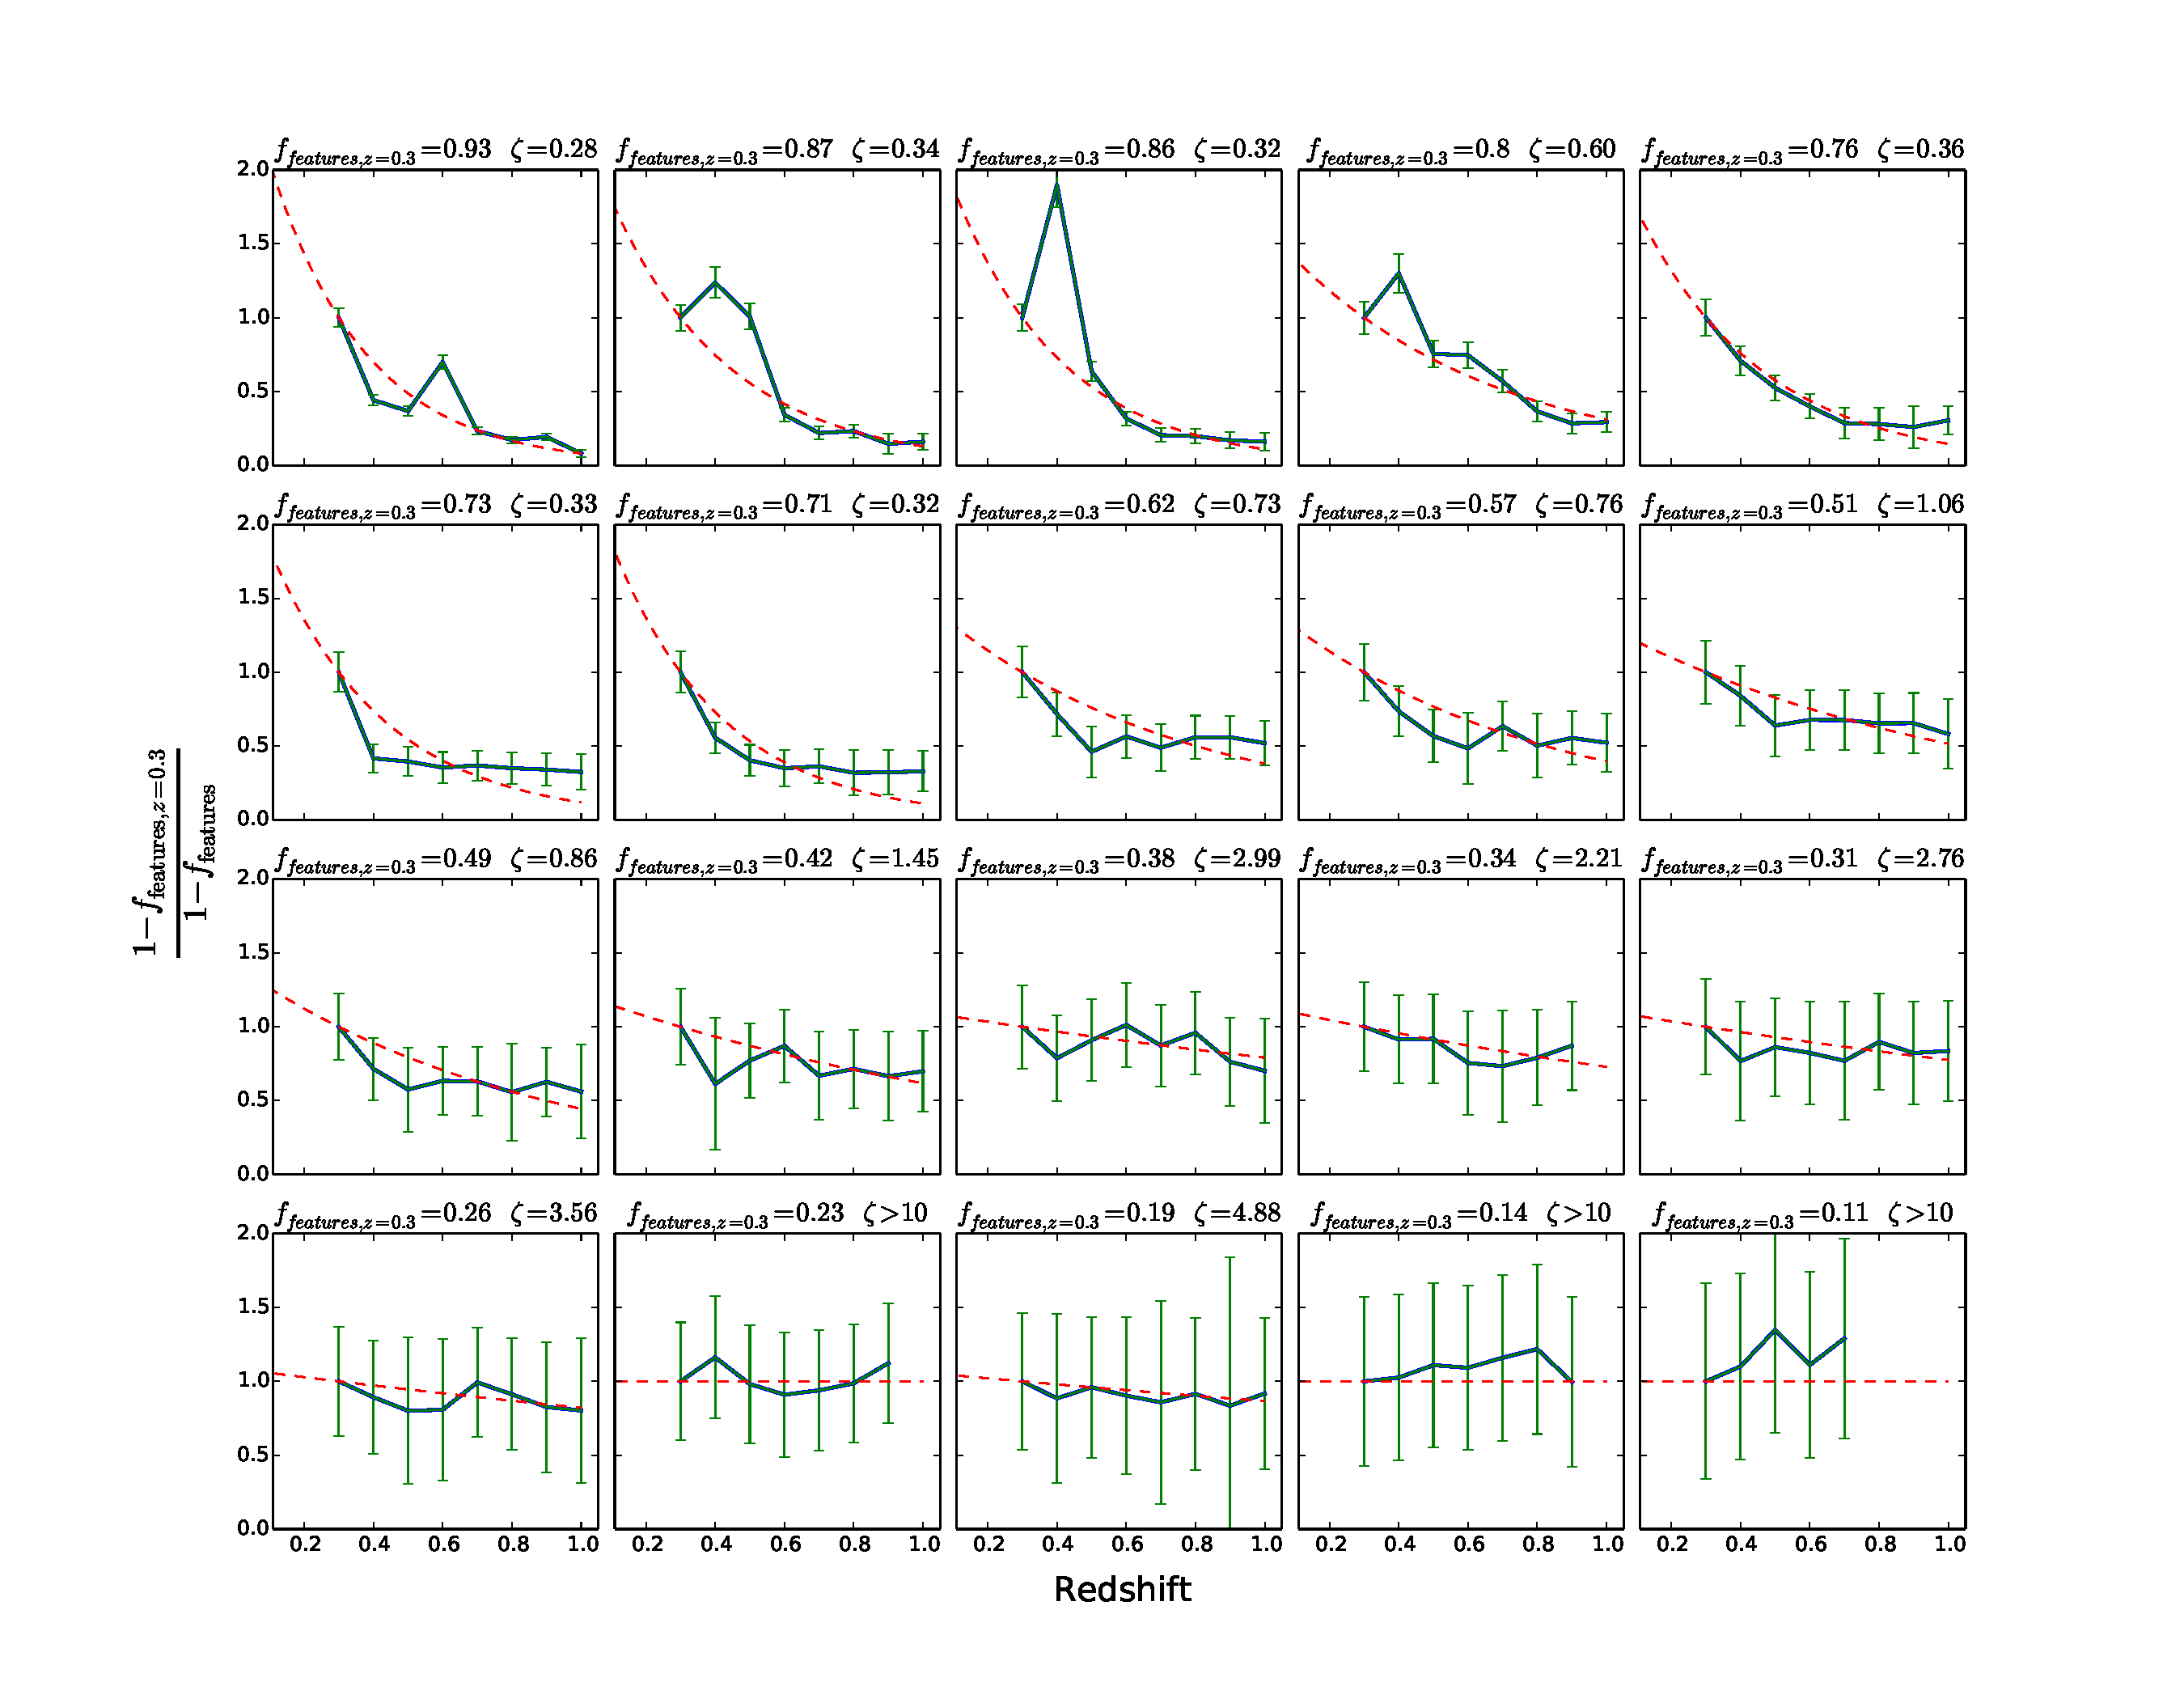
\includegraphics[width=\textwidth]{figures/zeta_examples_sorted.pdf}
\caption{Behaviour of the normalised, weighted vote fractions of features
visible in a galaxy ($f_\textrm{features}$) as a function of redshift in the
artificial \ferengi{} images. Galaxies in this plot were randomly selected from
a distribution with evolutionary correction $e=0$ and at least three detectable images 
in redshift bins of $z\ge0.3$. The displayed bins are sorted by \ffeaturesrest, 
labeled above each plot. Measured vote fractions (blue
solid line) are fit with an exponential function (red dashed line;
Equation~\ref{eqn:fzeta}); the best-fit parameter for $\zeta$ is given above
each plot.}


% Error bars are binomial for each f, symmetrised, then added in quadrature.
\label{fig:zeta_examples}
\end{figure*}



Equation~\ref{eqn:fzeta} is then fit to each galaxy in the ``correctable'' \ferengi{} sample, and $\zeta$ is measured for each. Figure~\ref{fig:zeta_examples} shows the best fit equations for 16 galaxies, and the $\zeta$ corresponding to the best fit is displayed with each galaxy. As it was assumed that surface brightness likely plays a role in the level of dropoff in \ffeatures{}, and hence the value of $\zeta$ which controls this dropoff, it is assumed that $\zeta$ follows a simple linear dependence with surface brightness:


\begin{equation}
\log_{10}(\hat\zeta) = \zeta_0 + (\zeta_1 \times \mu),
\label{eqn:zetafit}
\end{equation}

where $\hat\zeta$ is the correction factor applied to each galaxy. Figure~\ref{fig:zeta_mu} shows the relationship between the derived $\zeta$ values and the surface brightness $\mu$ of the \ferengi{} galaxies, which is fit with equation~\ref{eqn:zetafit}. The best-fit parameters to this linear fit from least-squares optimization are  $\zeta_0=0.50$, $\zeta_1=-0.03$. Interestingly, only a very weak surface brightness dependence is detected. It is difficult to determine from these data whether the weak detection is due to a true lack of dependence, or insufficient data (only 28 galaxies had sufficient data to accurately measure $\zeta$). 

\begin{figure}
\center
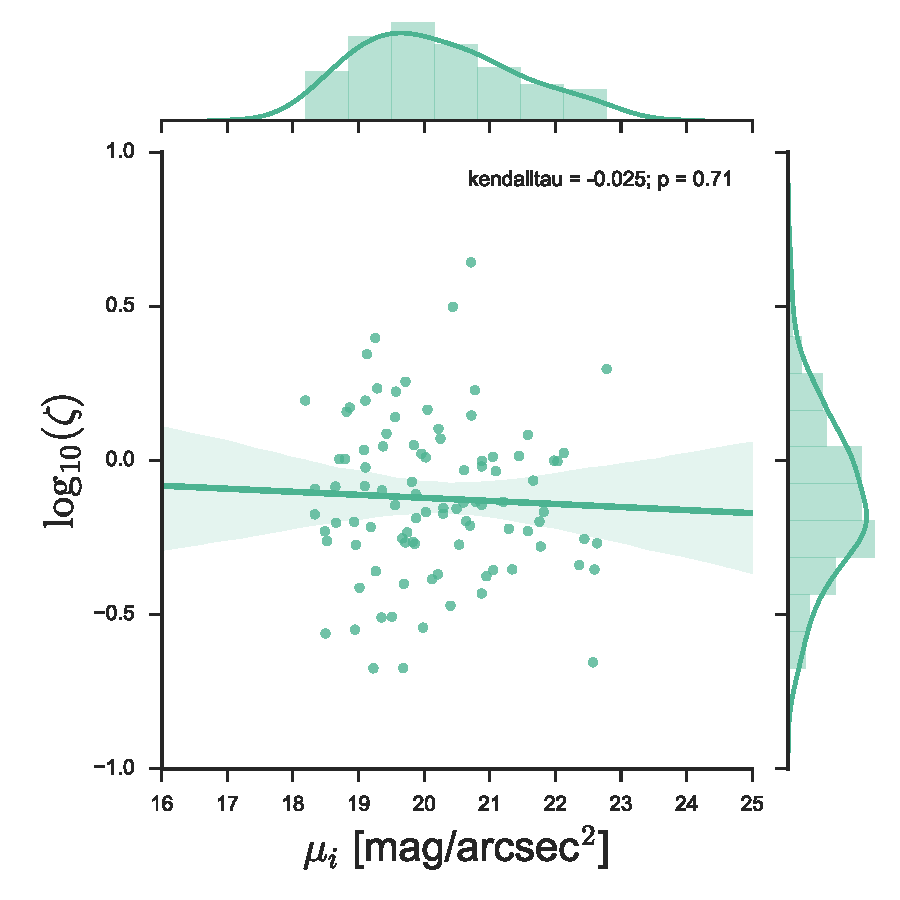
\includegraphics[width=0.5\textwidth]{figures/zeta_mu.pdf}
\caption{All fits for the \ferengi{} galaxies of the vote fraction dropoff
parameter $\zeta$ for \ffeatures{} as a function of surface brightness. This
includes only the simulated galaxies with a bounded range on the dropoff
($-10<\zeta<10$) and sufficient points to fit each function (28~original
galaxies, each with varying images artificially redshifted in one to eight bins over a range from $0.3\lesssim z_\mathrm{sim}\lesssim1.0$).}

\label{fig:zeta_mu}
\end{figure}


Using the $\zeta$ parameters measured in the \ferengi{} sample, a final debiased correction equation is derived to correct the \ffeatures{} vote fractions in the HST data:
\begin{equation}
f_\textrm{features,debiased} = 1 - (1 - f_\mathrm{features,weighted})e^{\frac{-(z-z_0)}{\hat\zeta}}
\label{eqn:fzeta_mod}
\end{equation}

\noindent where $f_\mathrm{features,weighted}$ is the weighted vote fraction, and $f_{\rm features,debiased}$ is bounded 
between $f_{\rm features,weighted}$ and 1. 



\subsubsection{Results and the NEI sample: limitations of the \ferengi{} simulated data}


\begin{itemize}
\item show table of HST sample breakdown~\ref{tab:hubble_debiasable}
\item show how above method only works for HST galaxies with z/mu corresponding to ferengi space~\ref{fig:eye_of_sauron}
\item discuss why ferengi can't completely replicate mu distribution of HST (cite Karen response to referee) 
\item discuss limits shown in~\ref{fig:correctable_fraction}
\end{itemize}




%Figure: showing correctable sample in  redshift/ffeatures space 
\begin{figure}
\center
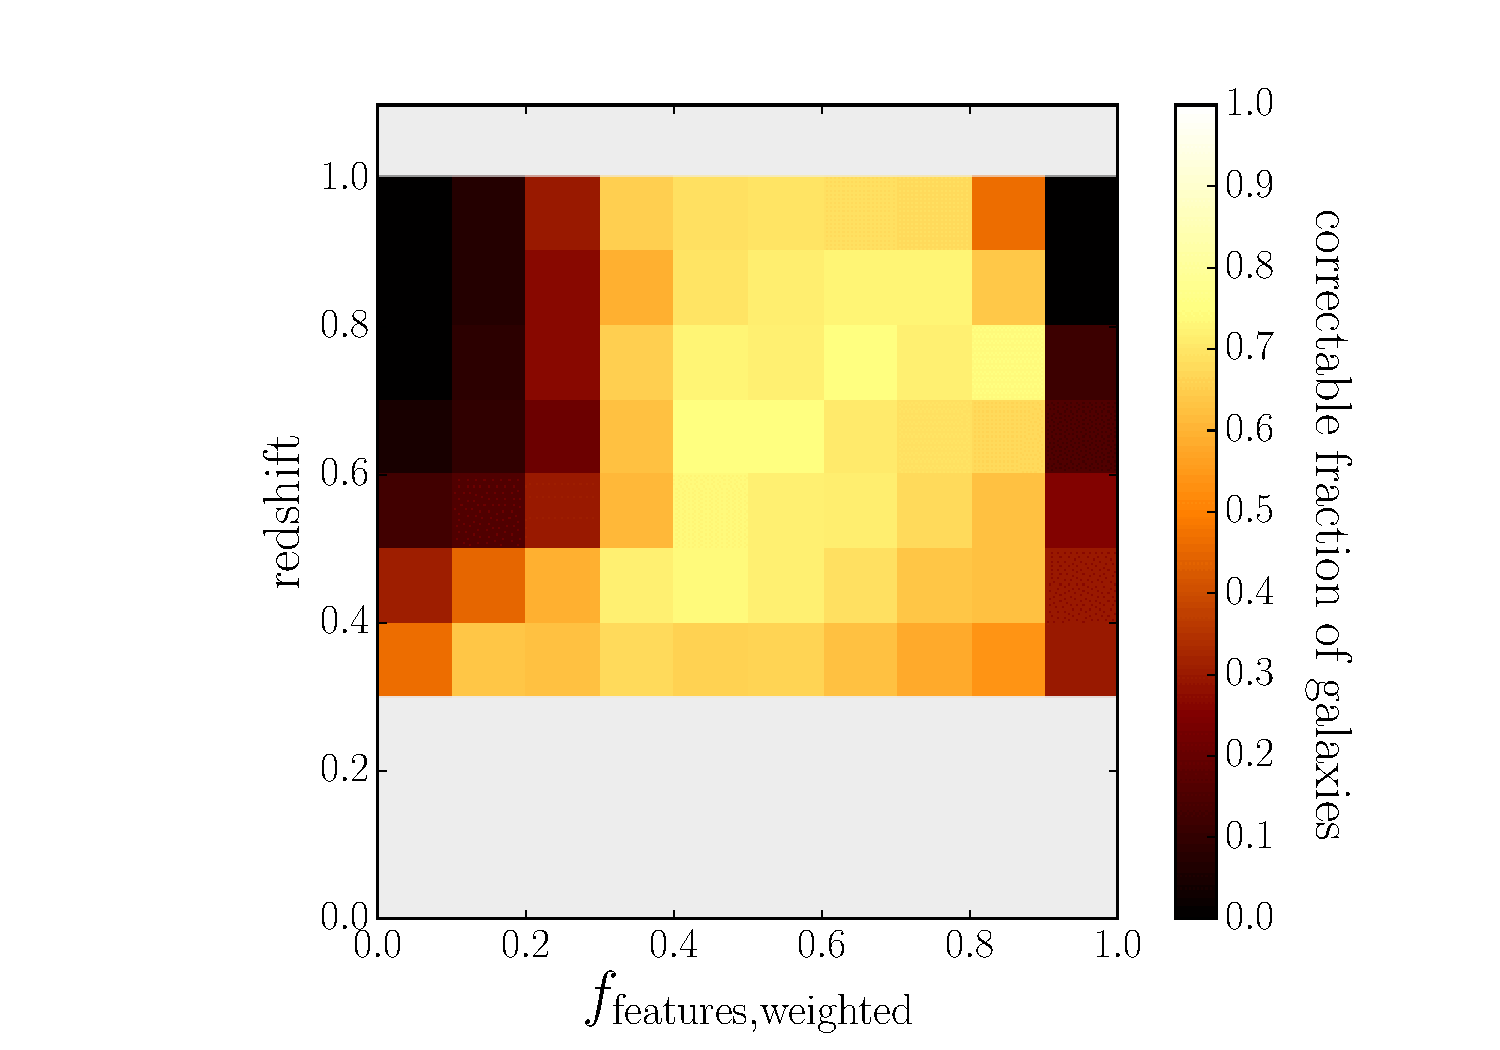
\includegraphics[width=0.5\textwidth]{figures/correctable_fraction.pdf}
\caption{Histogram showing the fraction of galaxies that have a finite correction
for the debiased vote fractions \ffeaturesdebiased{} as a function of \ffeatures{}
and redshift. The parameter space for corrections is limited to $0.3 \leq z \leq 1.0$
due to the sampling of the parent SDSS galaxies and detectability in the \ferengi{} images.
}
\label{fig:correctable_fraction}
\end{figure}

%Figure: compare z/mu distribution of hubble and ferengi sample
\begin{figure}
\begin{center}
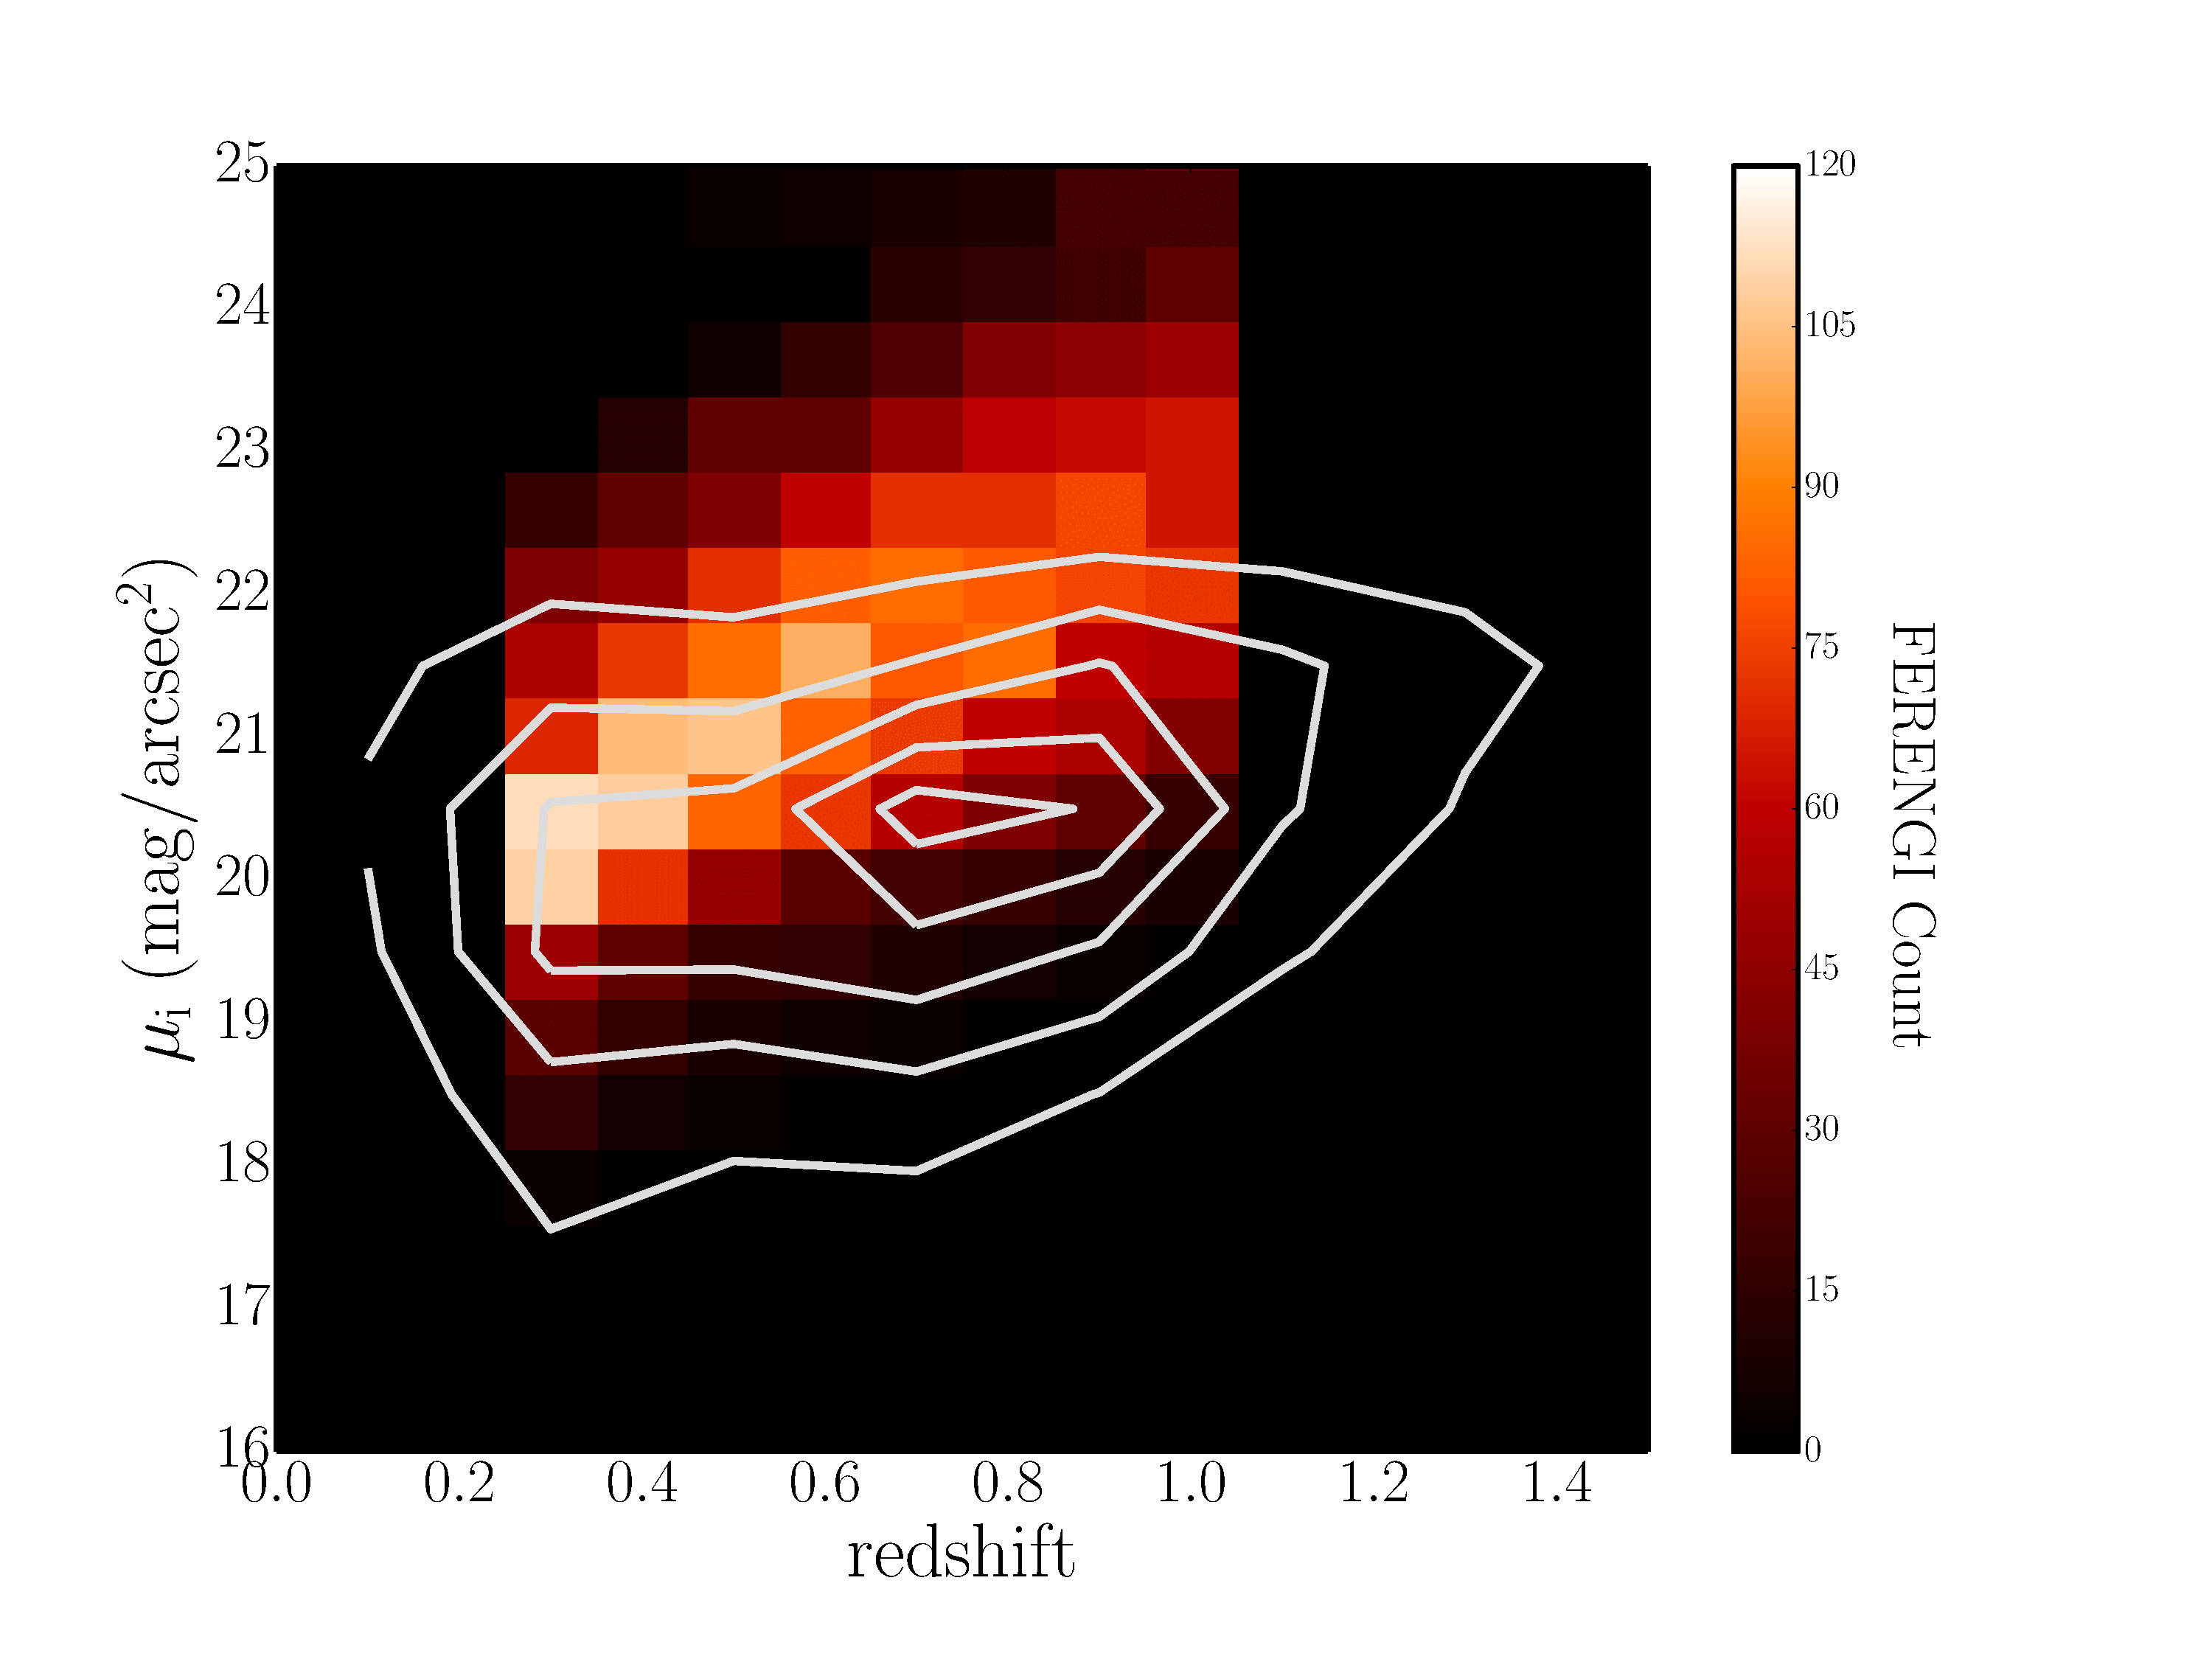
\includegraphics[width=0.5\textwidth]{figures/eye_of_sauron.pdf}
\caption{Surface brightness as a function of redshift for 3,449~\ferengi{}
images and the 102,548~\main{} galaxies with measured $\mu$ and $z$ values. The
colour histogram shows the number of \ferengi{} images as a function of $\mu$
and $z_{\rm sim}$. White contours show counts for the galaxies in the \main{}
sample, with the outermost contour starting at $N=1500$ and separated by
intervals of 1500.} 
\label{fig:eye_of_sauron}
\end{center}
\end{figure}
